% Chapter Template

\chapter{Karhunen-Lo\`{e}ve Transform} % Main chapter title

\label{Chapter3} 

\lhead{Chapter 3. \emph{Karhunen-Lo\`{e}ve Transform}}

Although use of mDLPs is one way to build physics into an energy basis, a more 
powerful approach is to use the Karhunen-Lo\`{e}ve transform (KLT)
\citep{Dony2001}.  This method goes by many names such as Proper 
Orthogonal Decomposition (POD) \citep{Buchan2013} and Principal Components 
Analysis (PCA) \citep{Dony2001}.  KLT has also been used for a variety of 
purposes, including model reduction in both fluid dynamics 
\citep{Sirovich1987} and reactor eigenvalue problems \citep{Buchan2013}.  
Additionally, KLT has been used in image compression \citep{Dony2001}.

The central goal of KLT is to approximate a discrete or continuous function 
$f(x)$ as a truncated expansion in an orthogonal basis whose functions yield the 
best possible $n$th-order approximation in terms of least-squares error for all 
values of $n$.  In some applications, such as image compression, the function 
$f$ is predetermined, e.g., a set of pixel values. For other applications, such 
as reduced-order modeling, the function $f$ is not known.  While details of its 
use in these applications may differ, KLT is fundamentally related to the 
singular value decomposition (SVD).

Suppose the global response matrix equations defined by \EQ{eq:globalrme} were 
solved using a full multigroup treatment and group-dependent boundary currents 
were reconstructed for each node from the resulting solution. Let $N$ denote the 
number of these currents, each of length $G$, the number of energy groups.  
Furthermore, let the $n$th current vector be denoted by $\mathbf{d}_n$.  These 
vectors, referred to as snapshots later in this work, are combined to form the 
matrix $\mathbf{D} \in \mathbb{R}^{G\times N}$, which is defined as $\mathbf{D} 
= [\mathbf{d}_1,\, \mathbf{d}_2,\, \ldots, \, \mathbf{d}_N]$. 

The present goal to to find a set of vectors that is the best representation 
of the columns of $\mathbf{D}$, i.e., the set of snapshots.  The full SVD 
of $\mathbf{D}$ is defined as
\begin{equation}
    \mathbf{D} = \mathbf{U} \bm{\Sigma} \mathbf{V}^{\intercal} \, ,
    \label{eq:svd}
\end{equation}
where $\mathbf{U} \in \mathbb{R}^{G\times G}$ is an orthogonal matrix of the
right-singular vectors, $\mathbf{V} \in \mathbb{R}^{N\times N}$ is an 
orthogonal matrix of left-singular vectors, and  $\bm{\Sigma} \in 
\mathbb{R}^{G\times N}$ is a matrix with diagonal elements $\sigma_{kk} \geq 0, 
\,  k = 1,\,2,\, \ldots,\, K = \min(G, N)$ arranged in decreasing order and 
zeros everywhere else. The $\sigma_{kk}$'s are referred to as singular values 
of the matrix $\mathbf{D}$.  The first $R=\text{rank}(\mathbf{D})\leq K$ 
singular values are positive (and the rank of a matrix is equal to the number 
of linearly independent columns). 

If instead of allowing all of the nonzero singular values into the construction 
of $\mathbf{\Sigma}$, only the largest $L$ values are used to define $\Sigma$, 
the problem space will be reduced.  \, \citet{eckart1936approximation} proved that 
the rank-$L$ matrix $\tilde{\mathbf{D}} \in \mathbb{R}^{G\times N}$ that 
satisfies
\begin{equation}
    \min_{ \substack{\tilde{\mathbf{D}} \in \mathbb{R}^{G\times N} \\ \text{rank}(\tilde{\mathbf{D}})=L }} 
    || \mathbf{D} - \tilde{\mathbf{D}} ||_F 
    \label{eq:frobnorm}
\end{equation}
is defined as
\begin{equation}
    \tilde{\mathbf{D}} = \tilde{\mathbf{U}} \tilde{\bm{\Sigma}} \tilde{\mathbf{V}}^{\intercal} \, ,
    \label{eq:svdL}
\end{equation}
where $\tilde{\mathbf{U}} \in \mathbb{R}^{G\times L}$ and $\tilde{\mathbf{V}} 
\in \mathbb{R}^{N\times L}$ contain the first $L \leq K$ columns of $\mathbf{U}$ 
and $\mathbf{V}$, the diagonal matrix $\tilde{\bm{\Sigma}} \in R^{L\times L}$ 
has nonzero elements equal to the first $L$ singular values of $\mathbf{D}$, and 
the Frobenius norm of a matrix $\mathbf{A}$ with elements $a_{gn}$ and columns 
$\mathbf{a}_n$ is defined as 
\begin{equation}
    ||\mathbf{A}||_F = \sqrt{\sum^G_{g=1} \sum^N_{n=1} a_{gn}^2} = \sqrt{\sum_{n=1}^N ||\mathbf{a}_n||^2_2 }\, .
\end{equation}
Therefore, the matrix $\tilde{\mathbf{D}}$ that satisfies \EQ{eq:frobnorm} 
provides 
a least-squares representation of the entire set of data contained in 
$\mathbf{D}$.  Equivalently, the columns of $\tilde{\mathbf{D}}$ are 
approximations of the columns of $\mathbf{D}$ with the minimum root mean square 
(RMS) error. 

% Now suppose that $G \geq N$ (this discussion applies equally well if $N$ is 
% greater than $G$ by simply taking the transpose of $\mathbf{D}$).  A 
% $G$-by-$(G-N)$ matrix $\tilde{\mathbf{U}}$ is constructed such that 
% $\hat{\mathbf{U}} = [\mathbf{U},\tilde{\mathbf{U}}]$.  Now $\hat{\mathbf{U}}$ 
% and $\mathbf{V}$ are nonsingular, so the rank of $\mathbf{D}$ is the same as the 
% rank of $\hat{\mathbf{U}}^{\intercal} \mathbf{D} \mathbf{V} = 
% \hat{\mathbf{\Sigma}}$ where
% \begin{equation*}
%     \hat{\mathbf{\Sigma}} = \left[ \begin{array}{c}
%         \mathbf{\Sigma}^{N\times N} \\
%         0^{(G-N)\times N} \end{array} \right] \, .
% \end{equation*}
% This formation leads to the so called rank-revealing form of the SVD, which 
% takes only the nonzero singular values to form $\mathbf{\Sigma}$.  This 
% formation allows for the lowest cost SVD and additionally, reveals the rank of 
% $\mathbf{A}$ to be equal to the number of nonzero singular values.  Using the 
% rank revealing SVD, the matrix $\mathbf{D}$ can be deconstructed to
% \begin{equation}
%     \mathbf{D} = \mathbf{U} \mathbf{\Sigma} \mathbf{V}^{\intercal} \, ,
%     \label{eq:SVD_of_D}
% \end{equation}
The KLT is designed to generate a set of orthogonal basis vectors that capture 
the most important information of the defining matrix.  In this case, that 
matrix is $\mathbf{D}$, so the singular vectors of a matrix capture the most
important information about the snapshots.  Thus, part of the KLT is to identify 
the singular values of the matrix $\mathbf{D}$.  By extension of \EQ{eq:svd}
\begin{equation}
    \mathbf{D}^{\intercal}\mathbf{D}  = \mathbf{V} \mathbf{\Sigma} 
    \mathbf{U}^{\intercal} \mathbf{U} \mathbf{\Sigma} \mathbf{V}^{\intercal} = 
    \mathbf{V} \mathbf{\Sigma}^2 \mathbf{V}^{\intercal} \, .
    \label{eq:find_eigenvalues}
\end{equation}
Thus the SVD of the quantity $\mathbf{D}^{\intercal}\mathbf{D}$ yields 
$\mathbf{V}$, which are the right-singular vectors of $\mathbf{D}$.  When 
using the SVD of the matrix $\mathbf{D}^{\intercal}\mathbf{D}$, the result 
is equivalent to the eigenvalue decomposition of 
$\mathbf{D}^{\intercal}\mathbf{D}$.  The eigenvalue decomposition is of a similar form to 
\EQ{eq:find_eigenvalues} and is given by
\begin{equation}
    \mathbf{D}^{\intercal}\mathbf{D} = \mathbf{B} = 
    \mathbf{Q}\mathbf{\Lambda}\mathbf{Q}^{-1}\, ,
    \label{eq:eval_decomp}
\end{equation}
where the columns of $\mathbf{Q} \in \mathbb{R}^{N\times N}$ are the 
eigenvectors of $\mathbf{B} \in \mathbb{R}^{N\times N}$, and $\mathbf{\Lambda} 
\in \mathbb{R}^{N\times N}$ contains the eigenvalues of $\mathbf{B}$ in 
decreasing order. 

From \EQ{eq:eval_decomp}, the eigenvectors contained in 
$\mathbf{Q}$ of the eigenvalue decomposition of $\mathbf{D}^{\intercal}\mathbf{D}$ are 
equivalent to the right
singular vectors of $\mathbf{D}$ with corresponding singular values contained in 
$\mathbf{\Sigma}$. Also important to note is that 
$\mathbf{D}^{\intercal}\mathbf{D}$ is a symmetric, square, real-valued matrix, 
which simplifies many linear algebraic computations and guarantees that the 
eigenvalue decomposition exists.  Furthermore, many algorithms exist to find eigenvalues and 
corresponding eigenvectors of symmetric matrices, which are quicker than computing the SVD of 
$\mathbf{B}$.

In short, we desire the information contained in the singular vectors of 
$\mathbf{D}$.  The singular vectors of $\mathbf{D}$ are equivalent to the 
eigenvectors of $\mathbf{B}$.  By taking only the $N$ largest eigenvalues and 
corresponding eigenvectors  of $\mathbf{B}$, the eigenvectors 
provide the best $N$th order least squares representation of $\mathbf{B}$, and 
correspondingly the least squares representation of $\mathbf{D}$.  By working 
with $\mathbf{B}$ instead of $\mathbf{D}$, many computations are quicker.

This approach leads to the simple implementation algorithm to find the basis 
functions, $P^i_{\text{KLT}}(:)$, first described by \citet{Meyer2002}, as 
follows. Form the data matrix, $\mathbf{D}$ as above.  Then the matrix 
$\mathbf{B} \in \mathbb{R}^{N\times N}$ is defined as
\begin{equation}
    \mathbf{B} = \mathbf{D}^{\intercal}\mathbf{D} \, .
    \label{eq:KLT}
\end{equation}
Now find the eigenvectors corresponding to the largest eigenvalues of the matrix $\mathbf{B}$,
\begin{equation}
    \label{eq:SVD_of_B}
    \mathbf{B} = \mathbf{Q}\mathbf{\Lambda}\mathbf{Q}^{-1}\, ,
\end{equation}
where $\mathbf{Q}$ from \EQ{eq:SVD_of_B} is equal 
to $\mathbf{V}$ 
from the SVD of $\mathbf{D}$ in \EQ{eq:svd}, and is thus the set of 
eigenvectors of 
$\mathbf{D}$. The eigenvectors $\mathbf{q}_j$ (columns of $\mathbf{Q}$ from 
\EQ{eq:SVD_of_B}), are 
then multiplied by the data matrix to form the basis vectors $P^j_{KLT}(:)$, 
i.e.,
\begin{equation}
    P^j_{KLT}(:) = \mathbf{D}\mathbf{q}_j \, ,
\end{equation}
which are subsequently orthonormalized.  Then an approximate representation of 
an arbitrary $N$-vector $\mathbf{f}$ in the basis is 
\begin{equation}
    \mathbf{f} \approx \sum_j a_j P^j_{KLT}(:) \, \quad \text{where} \quad a_j 
    = 
    \mathbf{f}^T P^j_{KLT}(:) \, .
    \label{eq:KLT_def}
\end{equation}
The form of \EQ{eq:KLT_def} is comparable to that of 
\EQS{eq:groupfluxmoments}{eq:groupcurrentcoefficients}.  The KLT is used to 
create a set of $N$ basis vectors that are best $N$th order approximation of 
the data to which the KLT applied.  In other words, the $k$th basis function is 
stretched such that the basis vector can best approximate a snapshot 
$\mathbf{d}$ when used in conjunction with all $i<k$ vectors of the basis set.  
Thus, the KLT maximizes the projection of a basis vector onto the data to 
which the KLT was applied.  This means that the KLT basis is constructed to 
obtain the most efficient basis functions for order reduction. For example, the 
most efficient storage for a zeroth 
expansion of a function is the function itself, which is an uninteresting use 
of KLT.  However, when instead applied to a set functions, KLT 
efficiently detects the prominent 
modes in the set.  In this case, the zeroth-order basis function 
typically resembles the average of the functions to which KLT is 
applied.

Defining the KLT basis vectors requires that values of the function to be 
expanded be known {\it a priori}.  For an application such as image compression,
those values are completely known.  However, for applications in reduced order 
modeling, knowledge of the true function to be expanded,
e.g., the group-dependent angular current, would require the full system to be 
solved, which may be impossible for sufficiently large models.  Additionally, 
if the complete solution is already known, there remains little need to 
approximate the solution. Therefore, an approximation must be made in order to 
sample values of the function to be expanded.  

For  time-dependent fluid dynamics, Sirovich proposed a method 
\citep{Sirovich1987} that is now known as the {\it method of snapshots} 
\citep{Buchan2013}. The method was used originally to produce reduced-order 
models for spatially-discretized, continuous-in-time models by computing the 
space-dependent solution only at discrete times. The resulting data, or matrix 
$\mathbf{D}$, is reduced significantly from the continuous case.

Again, the solution of the global response matrix equations should 
be avoided because it could be prohibitively large and would preclude the need 
for a basis expansion.  Thus, an effective basis set that can reconstruct 
the global solution without solving the global solution directly is sought.  
The true set of vectors $\mathbf{d}_n$ is assumed to be unavailable, so an 
alternative method to generate snapshot data is required. The implemented
approach is similar to traditional lattice physics methods in which a small, 
representative portion of the global domain (e.g., a many-group, two-dimensional 
assembly model) is used to generate an approximate global model (e.g., 
few-group, three-dimensional reactor model).  For KLT, small, ``snapshot model'' 
problems are solved from which group-dependent fluxes at various space and 
angle points are extracted as snapshot vectors.  These vectors become 
columns of an approximate $\mathbf{D}$, and KLT is constructed and applied as described.  
Since snapshot vectors do not represent the true solution space, optimality of 
KLT is not guaranteed. However, if the set of snapshots is sufficiently similar 
to the solution, then KLT can provide excellent results when applied to ERMM as 
an energy basis.

To illustrate application of KLT, reconsider the 10-pin example from 
\CHAPTER{Chapter2}.  The KLT approximation is applied 
to expand the known solution for the scalar flux, and its performance 
is compared to that of DLP and mDLP.  The data is arranged as 
the matrix $\mathbf{D} 
\in \mathbb{R}^{G\times N}$, where $G=44$ and $N=280$.  Following the algorithm 
described starting with \EQ{eq:KLT}, the basis function are constructed.  These 
basis functions can be observed in \FIG{fig:KLT_basis}.  Note that the 
zeroth-order function is approximately identical to the zeroth order from 
either type of mDLP.  It is in the remaining basis functions that KLT differs 
from mDLP.

\begin{figure*}[bt]
    \centering
    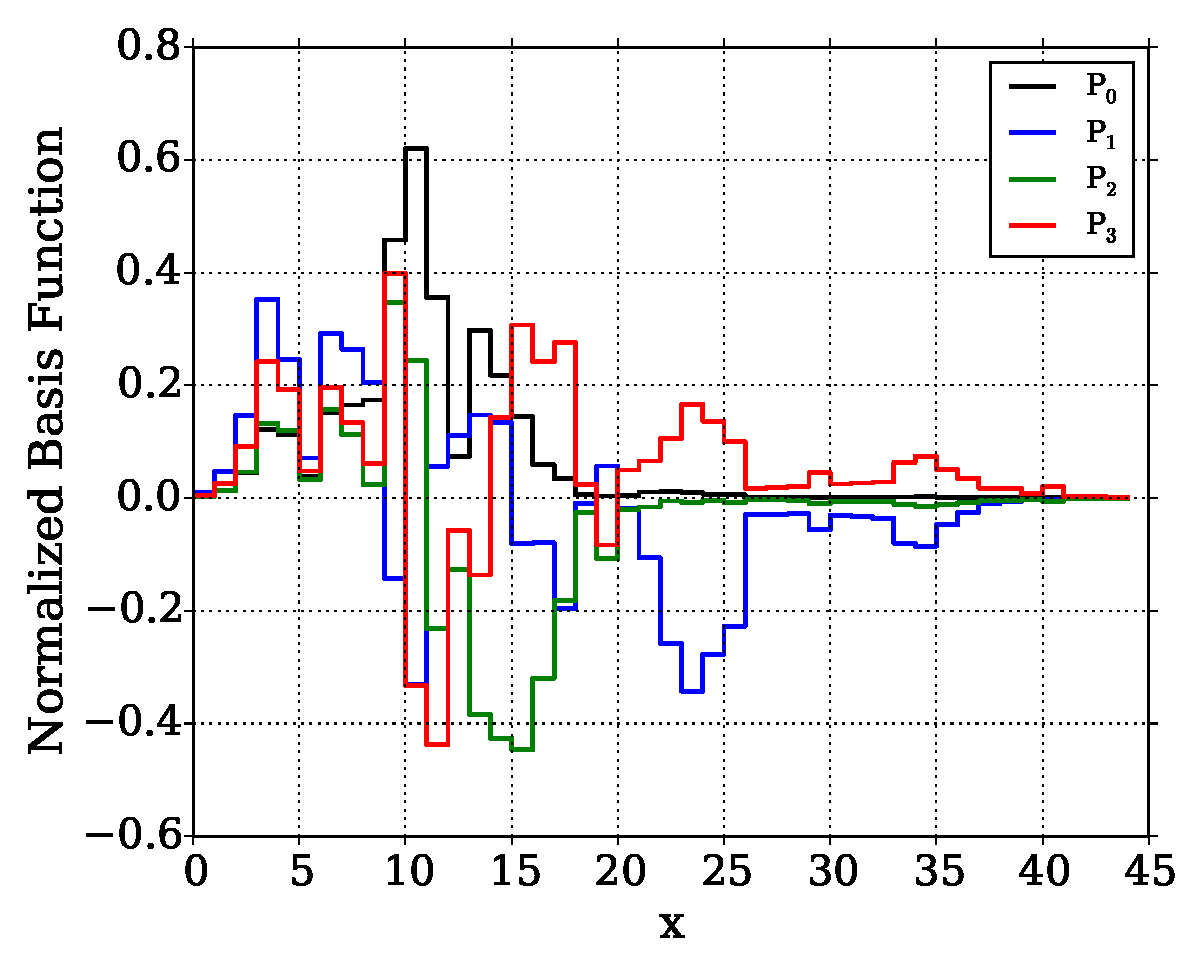
\includegraphics[trim=.1cm .25cm .1cm .4cm, clip=true,
    totalheight=0.35\textheight]{Figures/KLT_basis}
    \caption{Basis functions for the KLT applied to an example problem}
    \label{fig:KLT_basis}
\end{figure*}

The performance of the KLT basis set is shown in \FIG{fig:KLT_example}.  
Clearly, KLT outperforms DLP and mDLP for this example problem as KLT retains 
considerably more physics in the basis functions than mDLP can achieve.  
Also note 
that it takes considerably longer to compute the KLT basis function as compared 
to DLP or mDLP; however, the computation time for the basis generation of KLT 
is still orders of magnitude shorter than the time required to solve for the 
snapshot models or the test-problem itself.

\begin{figure*}[bt]
    \centering
    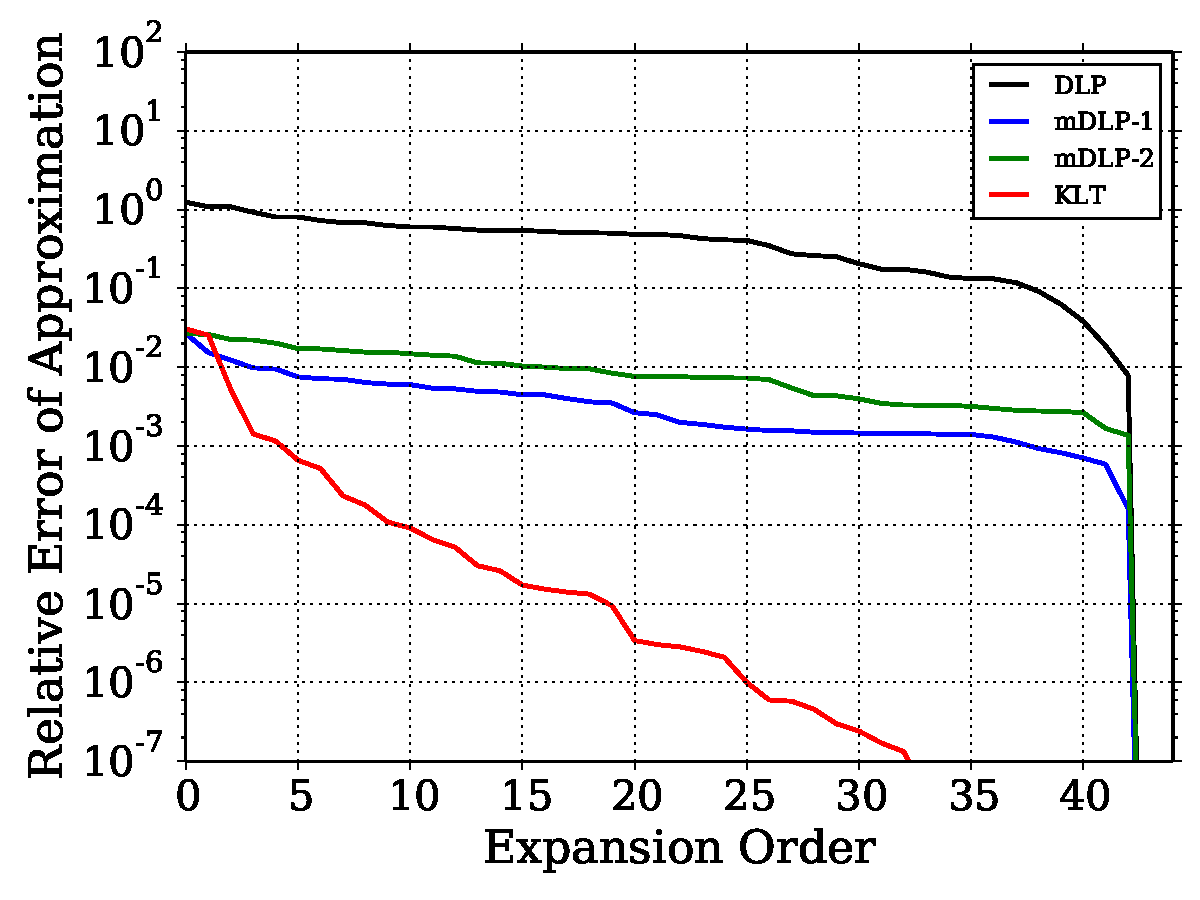
\includegraphics[trim=.1cm .25cm .1cm .33cm, clip=true,
    totalheight=0.35\textheight]{Figures/KLT_example}
    \caption{Relative error in the $L_2$ norm as a function of expansion order 
for 
KLT 
compared to other basis sets}
    \label{fig:KLT_example}
\end{figure*}